\documentclass[12pt]{article}
\usepackage[12pt]{moresize}
\usepackage[margin=1in]{geometry}

\usepackage{amsmath}
\usepackage{amssymb}

\usepackage{graphicx}
\usepackage{subcaption}

\usepackage{multirow} %Combining rows in tables
\usepackage{diagbox}  %Table box split in twain

\usepackage{algorithm}
\usepackage{algpseudocode}
\usepackage{alltt}

\usepackage{multicol}

\usepackage{amssymb} %\checkmark symbol

%\usepackage{hyperref}
%\usepackage[latin1]{inputenc}
%\usepackage{listings}
%\usepackage{scrextend}
%\usepackage{changepage} %Adjustwidth

 

\title{ComS 474\\Homework 2}
\author{Sean Gordon}
\date{Sep 28, 2020}

\begin{document}
\maketitle



\noindent 1) $x = [1.1, 2.2, 3.3, 1]^T$\\


\noindent 2) $w^Tx = [1.1, 0, 3.3, 0]^T > 1$, therefore the class is 1.\\


\noindent 3) {\large $\sum_{i-1}^{n}(W^Tx_i'' - C_i)^2$}, where $C_i$ is the class of $x_i$\\


\noindent 4) 


\noindent \hrulefill \\\pagebreak

%\begin{figure}[htbp]
%\centerline{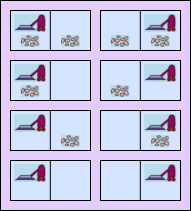
\includegraphics{Pics/ComS472_410.png}}
%\caption{Belief states recheable from initial 8 belief states.}
%\label{Belief states recheable from initial 8 belief states.}
%\end{figure}

\end{document}

















